\documentclass[a4paper]{article}

%% Language and font encodings
\usepackage[english]{babel}
\usepackage[utf8x]{inputenc}
\usepackage[T1]{fontenc}
\usepackage[section]{placeins}

%% Sets page size and margins
\usepackage[a4paper,top=3cm,bottom=2cm,left=3cm,right=3cm,marginparwidth=1.75cm]{geometry}

%% Useful packages
\usepackage{amsmath}
\usepackage{graphicx}
\usepackage[colorinlistoftodos]{todonotes}
\usepackage[colorlinks=true, allcolors=blue]{hyperref}

\begin{document}
\title{Thesis Proposal \\
\textbf{Self-calibrating Convolutional Neural Networks for Image Classification}}
\author{Duy Khoi Tran\\Matrikel Nr.: 9030205
}

\date{\parbox{\linewidth}{\centering%
  Master of Science in Autonomous Systems \endgraf\bigskip
  University of Applied Sciences Bonn-Rhein-Sieg \endgraf
  Advisor: Prof. Dr. Paul G. Plöger\endgraf
  Second Advisor: \color{red}???\color{black}\endgraf
  Third Advisor: \color{red}???\color{black}\endgraf
  \bigskip
  \today\endgraf\bigskip}}
\maketitle

\begin{abstract}
	
	 While training image classifiers, besides accuracy, the confidence of the network in their choices or predictions is also important. However, the representation of output uncertainties in modern convolutional neural networks, commonly Softmax, does not reflect actual reality and tends to be over-confident. Thus, they it needs calibrationg. \color{red} The aim of this project is to explore and establish the sufficient solutions for producing self-calibrating convolutional image classifiers, which calibrates its confidence in training phase and requires as little post-processing as possible. 

\end{abstract}

\section{Introduction}
\subsection{Background}

Modern Neural Networks are among the state-of-the-art solutions for many real-world complicated tasks. They have achieved outstanding performance in computer vision\cite{6993023}, natural language processing \cite{DBLP:journals/corr/LopezK17} and many other fields.

Apart from the overall prediction accuracy of a network, the confidence of the predictions should be taken into consideration. This information can help determine if the predictions should be trusted. This is of great relevance especially for high-stake applications such as medical diagnosis or self-driving car. A popular mechanism to quantify such information in classification task is the utilization of Softmax activation at the ouput of a network. This Softmax value of each class aims to convey directly the probabilities of the choices being correct. For example, if we have ten samples classified as a class with softmax value of 0.9, exactly nine out of ten samples should be correctly classified. If the predictions of a neural network are able to match its uncertainties to realitiy and estimate sufficiently the probability distribution of the training data, they are deemed well-calibrated \cite{DBLP:journals/corr/GuoPSW17, DBLP:thesis/calibration}. In an early research of binary classification, deep neural networks were thought to give well-calibrated results \cite{niculescu2005predicting}. However, recent works from Guo et al. shows that, with Softmax alone, modern deep neural networks, as highly accurate as they may be, are not well-calibrated \cite{DBLP:journals/corr/GuoPSW17}. This is attributed to popular deep learning practices such as depth increase, batch normalization and weight decay. In light of this fact, more researchers are starting to look for calibration methods to remedy this problem.

\subsection{Calibration methods}
Calibration methods are those that attempt to derive the accurate estimation of the class distribution from a network in arbitrary manner. However, they generally fall in to two categorizations: post-processing calibration and training phase calibration.

Post-processing calibration methods generally produce a mapping from the uncalibrated output of a pretrained network to calibrated probabilities. Methods in this type impose new learning tasks for the parameters of the mapping and, thus, require a dedicated calibration dataset that reflects the or the calibration can suffer from overfitting. Popular post-processing methods involve either putting the uncalibrated output into bins of calibrated probabilities \cite{Zadrozny:2001:OCP:645530.655658, Zadrozny:2002:TCS:775047.775151, DBLP:journals/corr/binning} or a variant of Platt scaling, Temperature Scaling \cite{Platt99probabilisticoutputs, DBLP:journals/corr/GuoPSW17, kuleshov2018accurate} that learns a regression model based on various types of loss \cite{mozafari2018new}.Post-processing caibration methods are relatively well-studied and intensively evaluated \cite{DBLP:thesis/calibration}. Temperature scaling has been established as the de facto method and acts as a baseline for both types of methods.

Training phase calibration is not as mature but is garnering a lot of research attention due to the elimination of output adjustment after training. This method type dominated by methods with Bayesian formalism \cite{lakshminarayanan2017simple}, in which prior distribution of weights are involved and the posterior distribution can be approximated using various approaches such as Laplace approximation \cite{mackay1999bayesian}, Markov chain Monte Carlo \cite{Neal:1996:BLN:525544} and variational Bayesian methods \cite{Blundell:2015:WUN:3045118.3045290, NIPS2011_4329, pmlr-v48-louizos16}. Other diverse popular directions involve ensemble of models \cite{Gal:2016:DBA:3045390.3045502, lakshminarayanan2017simple}, modification of losses or activation \cite{DBLP:journals/corr/abs-1810-11586, DBLP:journals/corr/abs-1810-01861}, similarity metrics \cite{DBLP:journals/corr/abs-1803-04765} or self-learning post-processing parameters \cite{Neumann18c}.

\color{red}Although the research volume for training phase calibration is quite substantial, there are some problems. The research works draw vague connections to each other. Their evaluation often use either different dataset and/or metrics depending aiming for potentially different aspects (out-of-distribution detection, robustness against adversarial attacks, etc.) Thus, a sufficient comparative evaluation can be challenging to produce from the literature.   

\subsection{Goal of the thesis}

The aim of this thesis project is to produce the aforementioned comparative evaluation of methods for self-calibrating convolutional neural networks for Image Classification. This work is inspired by the Master's thesis of Markus Kängsepp \cite{DBLP:thesis/calibration} that focuses solely on post-processing. The evaluation will be done accross multiple metrics, which include novel ones proposed alongside a few methods \cite{NIPS2018_7798, DBLP:journals/corr/abs-1709-09844}, and determine or develop the most suitable calibration method(s) in term of robustness, accuracy cost, computational cost, etc. to be applied in practical deep learning project. This project is based on the Master's Thesis of Markus Kängsepp \cite{DBLP:thesis/calibration} focusing on post-processing convolutional neural networks in the context of image classification. Attempts at novelty will also be taken in the form of experimenting self-learning variants of existing post-processing methods similar to the works of \cite{Neumann18c}. The product of this thesis should assist in the creation of Aptiv's deep learning framework for generating highly accurate and trustworthy intelligent systems.

\section{Methodology}

In order to fulfill the goals of the project, the prominent training-phase calibration methods will be chosen and implemented in Tensorflow Python. The implementations will be applied in training identical popular convolutional neural networks with common image datasets using the same configurations, unless otherwise specified. The performance and other relevant aspects of the trained networks will be evaluated accross multiple metrics, which include but not limited to Expected Calibration Error, Maximum Calibration Error, Negative Log Likelihood, Brier Score \cite{1950MWRv781B} and Trust Score \cite{NIPS2018_7798}.

For methods with Bayesian formalism, Tensorflow Probability might be used. Tensorflow Probability \cite{TensorProb} is a Tensorflow extension that allows distribution definition and sampling process in computational graph. From these capabilities, weights and other parameters can be represented as samples of a distributions and facilitate Bayesian modelling.

For experimentation of self-learning variants of post-processing methods, possible ideas are as below:
\begin{itemize}
	\item \textbf{Histogram Binning} \cite{Zadrozny:2001:OCP:645530.655658}: This class of non-parametric methods divide uncalibrated predictions into mutually exclusive intervals with a confidence score. With a sufficiently big and reflective calibration set, the bounds of these intervals can be calculated. In this thesis, experiementation will be done to learn these bounds during training providing the minibatch is sufficiently big and the number of bins is relatively low.
	\item \textbf{Parametric methods}: Attempts to make the neural networks learn the calibrating parameters during training will be made similar to the works of \cite{Neumann18c}.
\end{itemize}
There are other classes of post-processing methods that might be further examined and applied directly in training.

\color{black}

\section{Project Plan}
\subsection{Work packages}
In conducting the project, the following work packages will be handled:
\begin{itemize}
	
\item WP1: Literature research.
\item WP2: Methods implementation and model training.
\item WP3: Adjusting, testing of models.
\item WP4: Results extraction and Thesis report writing.
	
\end{itemize} 
All of these workpackages will be somewhat carried out in parallel.
\subsection{Schedule}
An estimated time line for the execution of the project can be seen in Figure \ref{fig:schedule}
\begin{figure}
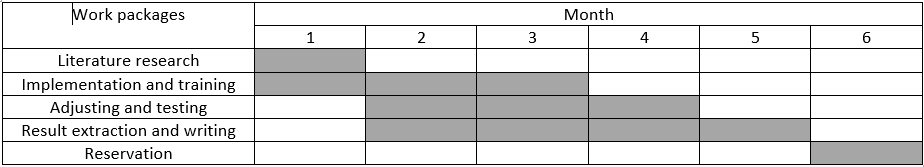
\includegraphics[width=1\textwidth]{gant.png}
\caption{Estimated schedule}
\label{fig:schedule}
\end{figure}

\subsection{Milestones}
\begin{itemize}
	\item Literature research leading to a survey of convey the landscape of self-learning convolutional neural network calibration
	\item Complete Python implementation of the calibration and the creation of neural network architecture with the methods applied.
	\item Sufficient empirical results that can reach to conclusive statements
	\item Establishment of the most suitable calibration methods
\end{itemize}

\section{Deliverables}
Minimum Deliveries:
\begin{itemize}
\item Minimum:
\begin{itemize}
\item A survey involving the analysis of the state-of-the-art in neural network calibration.
\item A theoretical comparative evaluation based on information from the researched literature.
\item Establishment of the most suitable calibration methods based on this evaluation.
\end{itemize}
\item Expected:
\begin{itemize}
\item Complete Python implementation of the calibration and the creation of neural network architecture with the methods applied.
\item Sufficient empirical results and derication of relevant observations.
\item Establishment of the most suitable calibration methods from the empirical data.
\end{itemize}
\end{itemize}


\bibliographystyle{alpha}
\bibliography{sample}

\end{document}